\subsubsection{\emph{Scenarios View}}
\label{subsubsec:use-case-view}

\emph{Scenarios View} menunjukkan perilaku sistem dari sudut pandang pengguna melalui pemodelan \emph{use case}. \autoref{fig:bpmn-to-be} menunjukkan \emph{Business Process Model and Notation} (BPMN) untuk \emph{use case} utama sistem, yaitu \emph{share-extract-save}. BPMN ini menunjukkan perbedaan alur kerja dari BPMN sistem saat ini (\emph{As-Is}) yang telah ditunjukkan pada \autoref{sec:analisis-kondisi-saat-ini}. Proses manual yang perlu dilakukan pengguna mulai dari mengekstrak data hingga menyimpan hasil pencatatan pengeluaran ke dalam aplikasi telah diotomatisasi pada sistem yang diusulkan.

\begin{figure}[htbp]
    \centering
    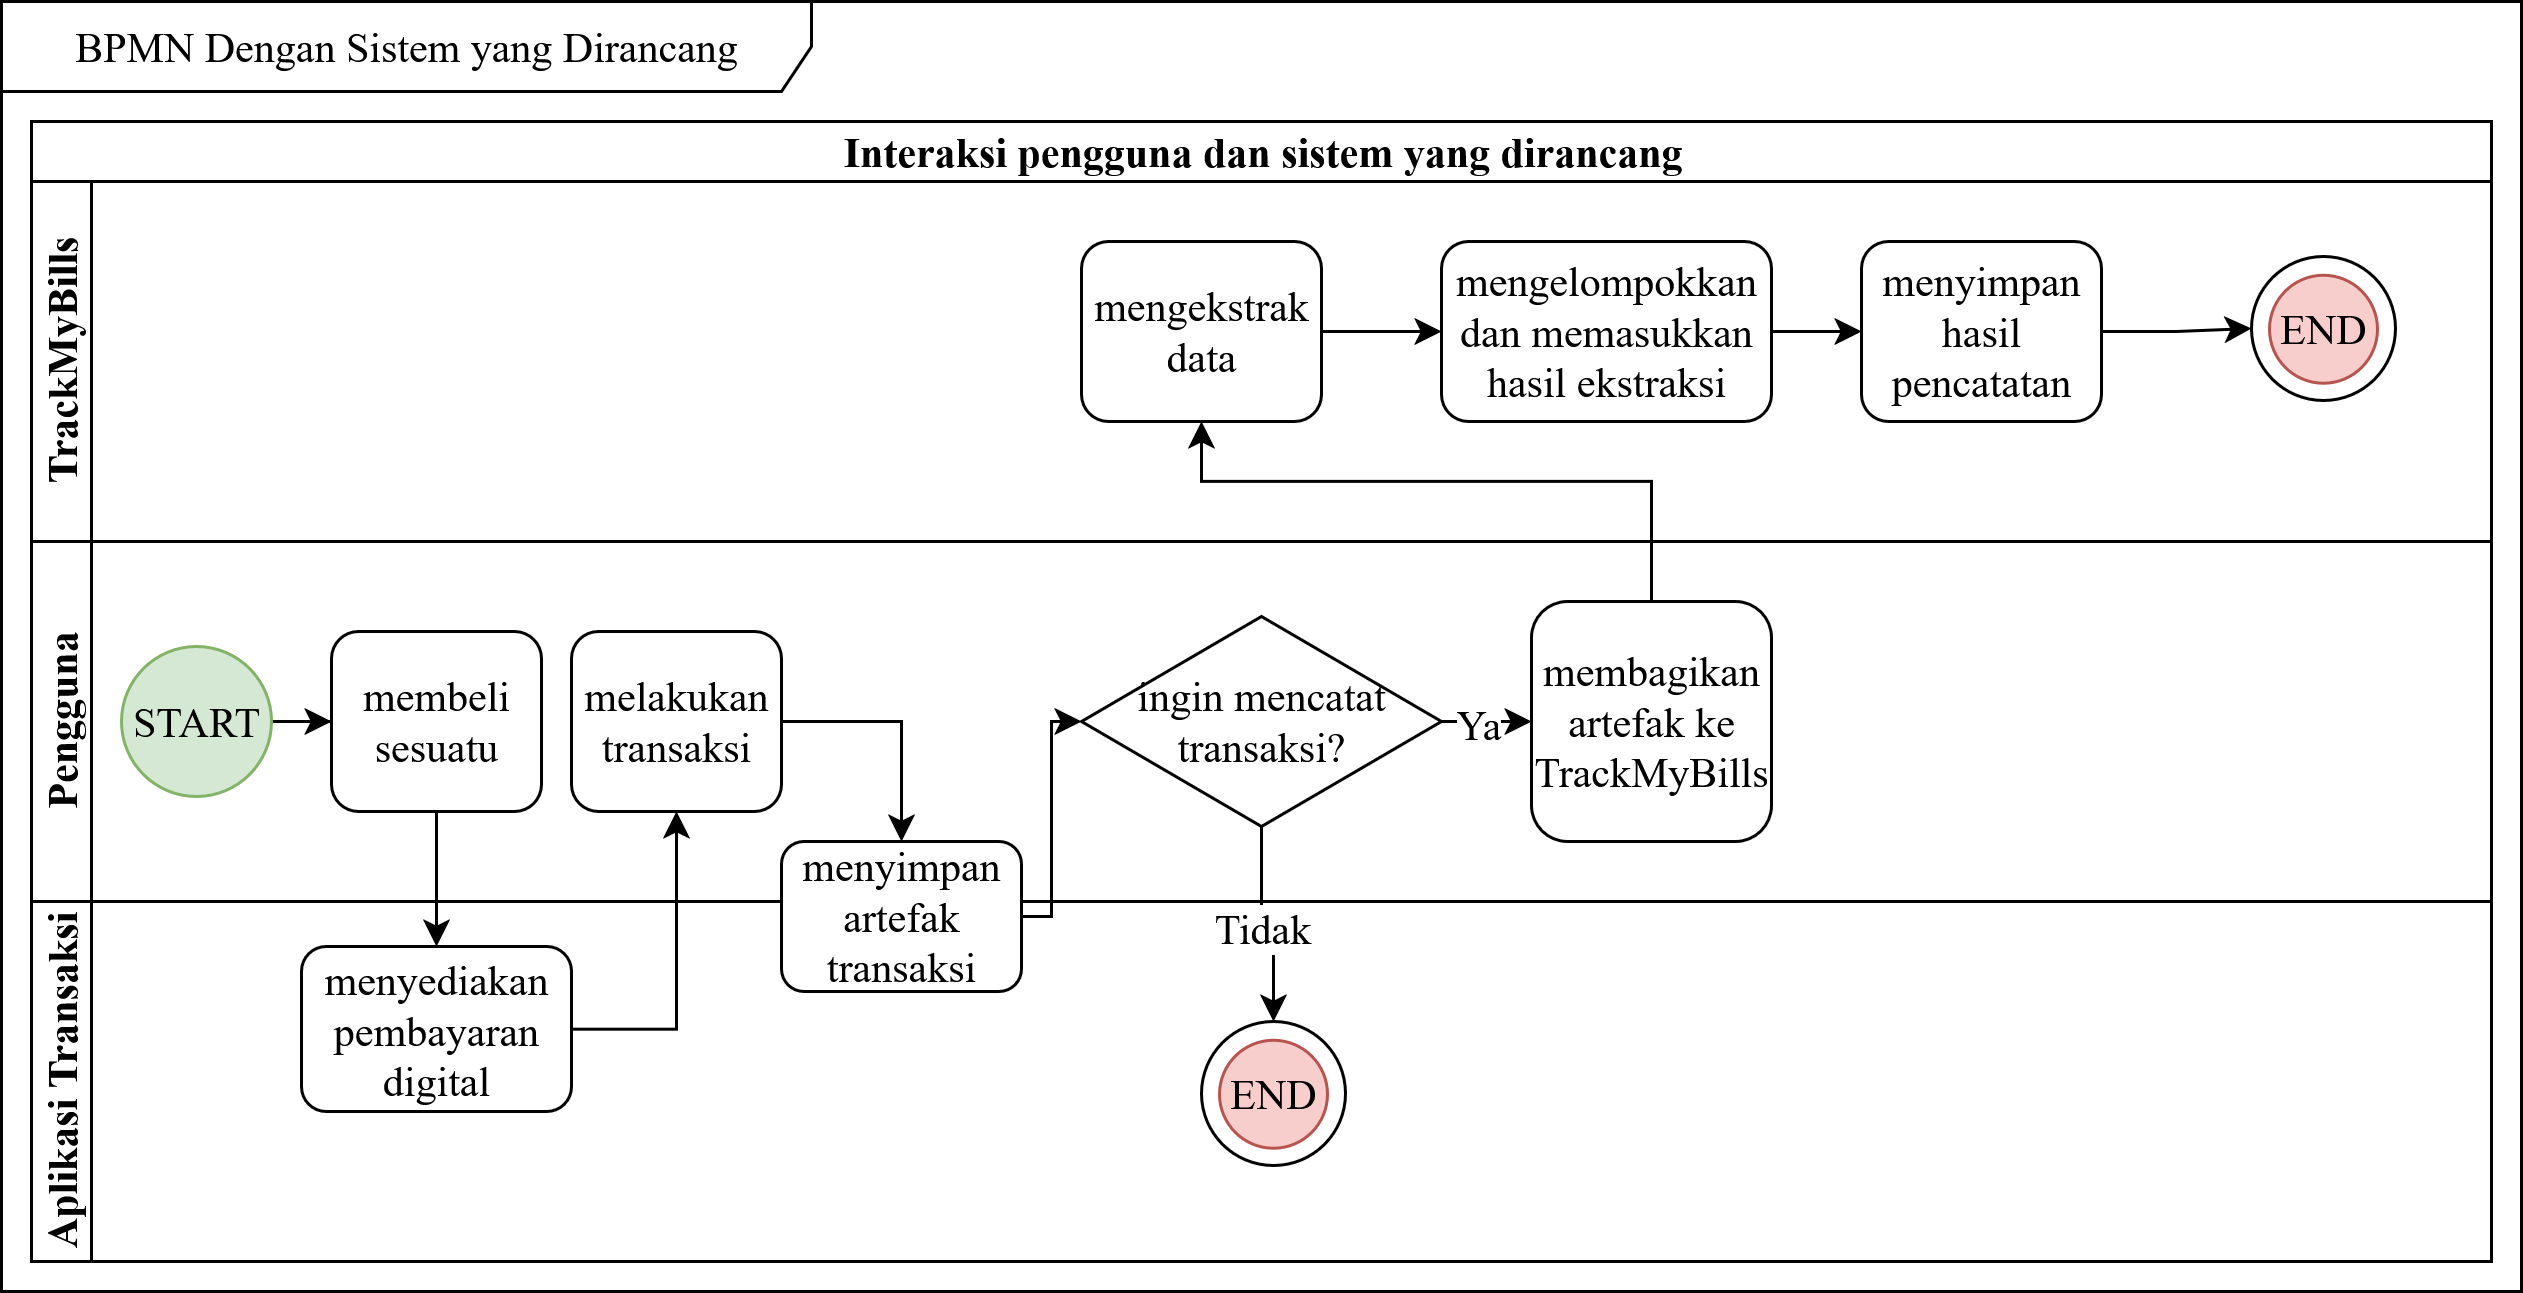
\includegraphics[width=1\textwidth]{images/To-be.png}
    \caption{BPMN untuk \emph{use case} utama sistem (\emph{share-extract-save})}
    \label{fig:bpmn-to-be}
\end{figure}

\begin{figure}[htbp]
    \centering
    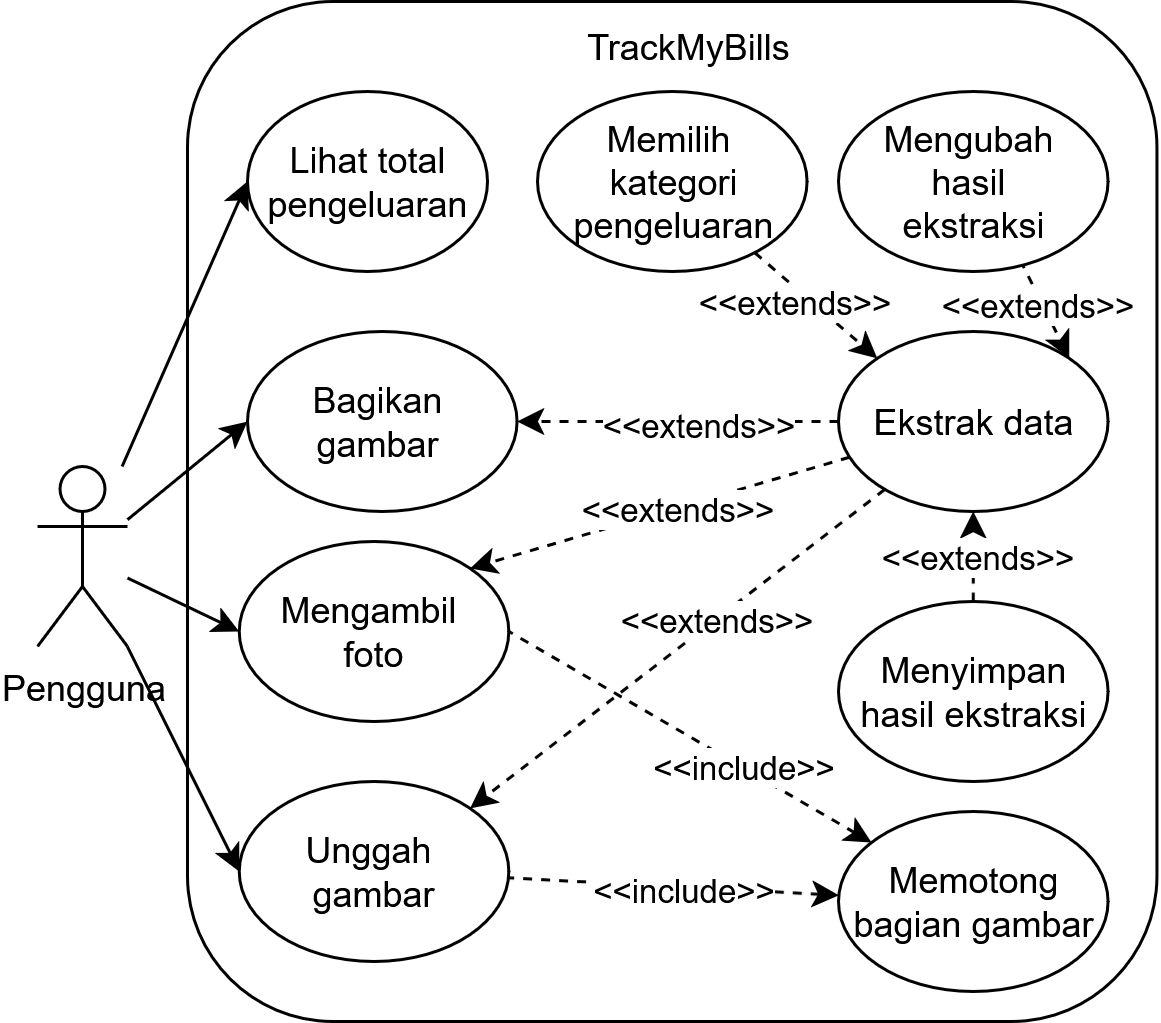
\includegraphics[width=.7\textwidth]{images/use-case-diagram.png}
    \caption{\emph{Use case diagram} sistem pencatatan pengeluaran berbasis \emph{mobile}}
    \label{fig:use-case-diagram}
\end{figure}